\documentclass{article}
\usepackage{amsmath,amssymb}
\usepackage{breqn}
\usepackage{graphicx}
\usepackage[left=1in,right=1in,top=1in,bottom=1in]{geometry}
\usepackage{cleveref}

\makeatletter
\newcommand*{\declarecommand}{%
  \@star@or@long\declare@command
}
\newcommand*{\declare@command}[1]{%
  \provide@command{#1}{}%
  \renew@command{#1}%
}
\makeatother

\declarecommand{\x}{{\mathbf{x}}}
\declarecommand{\p}{{\mathbf{p}}}

\declarecommand{\u}{{\mathbf{u}}}
\declarecommand{\U}{{\mathbf{U}}}
\declarecommand{\grad}{\nabla}
\declarecommand{\Wi}{\textnormal{Wi}}
\declarecommand{\Id}{\mathbb{I}}
\declarecommand{\f}{{\mathbf{f}}}
\declarecommand{\F}{{\mathbf{F}}}
\declarecommand{\n}{{\mathbf{n}}}
\declarecommand{\X}{{\mathbf{X}}}
\declarecommand{\b}{{\mathbf{b}}}
\declarecommand{\a}{{\mathbf{a}}}
\declarecommand{\bmu}{{\boldsymbol{\mu}}}
\declarecommand{\tS}{{\tilde S}}

\begin{document}

\section{The Bingham closure}

The Bingham closure is given by:
\begin{equation}
    S(\x) = \int\psi_B(\x,\p)\p\p\p\p\,d\p,
\end{equation}
where the Bingham distribution $\psi_B(\x,\p)$ is defined by the constraints that:
\begin{subequations}
    \begin{align}
        \int\psi_B(\x,\p)\,d\p      &= \phi(x),  \\
        \int\psi_B(\x,\p)\p\p\,d\p  &= D(\x),
    \end{align}
\end{subequations}
where $\phi$ and $D$ are the zeroth and second moments with respect to the true distribution function $\psi$. We assume that $\psi_B(\x,\p)$ takes the form:
\begin{align}
    \psi_B(\x,\p) = Ae^{B:\p\p}.
\end{align}
Given $\phi(\x)$ and $D(\x)$, our goals is to find the coefficients $A$ and $B$. Because $B$ only appears contracted against a symmetric matrix, it is sufficient to assume that $B$ is symmetric. In fact, we will see that our goal is even simpler than this: we will only be interested in computing $S:E$ and $S:D$, where $E=\grad\u+\grad\u^\intercal$. The purpose of this package is to provide optimized routines for computing these contractions. This documentation describes how the package works.

\section{The Bingham Closure in 2D}

\subsection{A simple formula for the closure}

From Chaubal and Leal, $B$ and $D$ are diagonalized in the same frame. We assume that we are in this frame; and compute the closure here. We will clean up details afterwards. In this frame, we have that:
\begin{subequations}
    \begin{align}
        1 &= \int_0^{2\pi}Ae^{\lambda_0\cos^2\theta + \lambda_1\sin^2\theta}\,d\theta,   \\
        \mu_0 &= \int_0^{2\pi}Ae^{\lambda_0\cos^2\theta + \lambda_1\sin^2\theta}\cos^2\theta\,d\theta,   \\
        \mu_1 &= \int_0^{2\pi}Ae^{\lambda_0\cos^2\theta + \lambda_1\sin^2\theta}\sin^2\theta\,d\theta,
    \end{align}
\end{subequations}
Note we have assumed here that $\phi=1$. $\mu$ and $\lambda$ are the eigenvalues of $D$ and $B$ respectively, with $\mu_0>\mu_1$. We note that $\lambda$ can only be fixed up to an additive constant: to see this, let $\lambda_0$ and $\lambda_1$ solve the above equations.  Then letting $\tilde\lambda_i=\lambda_i+C$ for $i=0,1$, we have:
\begin{equation}
    \int_0^{2\pi}Ae^{\tilde\lambda_0\cos^2\theta + \tilde\lambda_0\sin^2\theta}f(\theta)\,d\theta = \int_0^{2\pi}Ae^{C}e^{\lambda_0\cos^2\theta + \lambda_1\sin^2\theta}f(\theta)\,d\theta,
\end{equation}
which simply changes the definition of $A$. We can choose a convenient choice of $C$ then; it is convenient to choose $C$ so that $\lambda_0 + \lambda_1 = 0$. Then we have that:
\begin{subequations}
    \begin{align}
        1 &= \int_0^{2\pi}Ae^{\lambda_0(\cos^2\theta - \sin^2\theta)}\,d\theta,   \\
        \mu_0 &= \int_0^{2\pi}Ae^{\lambda_0(\cos^2\theta - \sin^2\theta)}\cos^2\theta\,d\theta.
    \end{align}
\end{subequations}
Exploiting the trig identity that $\cos^2\theta-\sin^2\theta=\cos(2\theta)$, and because:
\begin{equation}
    \int_0^{2\pi}e^{\lambda_0\cos(2\theta)}\,d\theta = 2\pi I_0(\lambda_0),
\end{equation}
we find that
\begin{equation}
    A = \frac{1}{2\pi I_0(\lambda_0)},
\end{equation}
where $I_v$ is the modified Bessel function of the first kind. Thus we find:
Now we're down to the single equation:
\begin{equation}
    \mu_0 = \frac{1}{2\pi I_0(\lambda_0)}\int_0^{2\pi}e^{\lambda_0\cos(2\theta)}\cos^2\theta\,d\theta.
\end{equation}
Evaluating this final integral and simplifying gives:
\begin{equation}
    2\mu_0 = 1 + \zeta(\lambda_0),
\end{equation}
where we have defined $\zeta(x)=I_1(x)/I_0(x)$. Thus to find $\lambda_0$ given $\mu_0$, we simply need to solve this nonlinear equation for $\lambda_0$.

\subsection{Solution of the closure equation and numerical issues}

In this section we consider the issues with solving the nonlinear equation:
\begin{equation}
    2\mu = 1 + \zeta(\lambda)
\end{equation}
for $\lambda$, given $\mu\in[0.5,1.0]$. Note that $\mu_0$, the largest eigenvalue, must live in this range becuase it is the largest eigenvalue and the eigenvalues sum to $1$. The fundamental problem with simply throwing a naive Newton solver at this equation is that as $\mu\to1$, $\lambda\to\infty$. While not a problem in and of itself, $\zeta(\lambda)$ is the ratio of $I_1(\lambda)$ and $I_0(\lambda)$. Both of these functions diverge exponentially fast as $\lambda$ gets large, and so naive evaluation of the ratio fails. Nevertheless, their ratio converges to $1$: our primary challenge is to find a way to evaluate $\zeta$ stably for large arguments. Fortunately, we are in luck! As it turns out, we can write:
\begin{equation}
    I_\nu(z) = \frac{e^z}{\sqrt{2\pi z}}\mathcal{P}_\nu(z),
\end{equation}
where $\mathcal{P}_\nu(z)$ is a power series in $z^{-1}$ that converges for sufficiently large $z$. Our strategy is clear, then. For small arguments, we can evaluate $\zeta$ directly. For larger arguments, we compute $\zeta$ by:
\begin{equation}
    \zeta(\lambda) = \mathcal{P}_1(\lambda)/\mathcal{P}_0(\lambda).
\end{equation}
In my numerical experiments, the power series $\mathcal{P}_0$ and $\mathcal{P}_1$ converge rapidly when the argument is at least $20$, and direct evaluation has no issues for this size argument. We thus evaluate $\zeta$ directly for $|\lambda|\leq20$, and indirectly via the power series representations for $|\lambda|>20$.


Cool.  Now this works well enough. And even better, we have a really fast way to solve this: brute force solve over a range of $\mu_0$, and then we just have a 1D regular interpolation problem to get $\lambda_0$. Once $\lambda_0$ is known, then we know $\lambda_1$, and rotating back (we already did the Eigendecomposition of $D$, and since $D$ is real and symmetric, we've got the rotation matrices. This gives us $B$, and now we can directly calculate the elements of $S$ and compute the various contractions.\\

Alas, there still seems to be a problem. As $\mu_0\to1$, we have that $\lambda_0\to\infty$. So, the whole thing goes to hell when you approach an aligned state. See \Cref{fig:problem}. Okay, I think I've fixed this now. There was a bug in my code, which drove things really to aligned states instead of keeping them away from them, AND $S_{0000}$ is much better behaved that $\lambda_0$ itself, so it is useful to interpolate that instead of $\lambda_0$. See the next section for details.
\begin{figure}
    \centering
    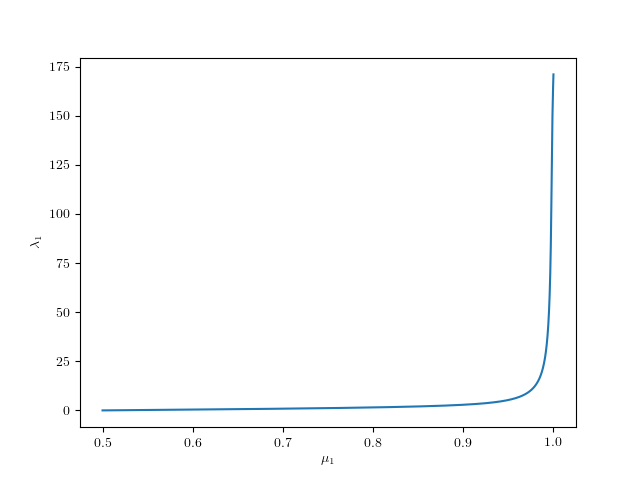
\includegraphics[width=0.8\textwidth]{problem}
    \caption{Blowup of $B$ as $D$ approaches a nematically aligned state. (Sorry, I switched notation. The $x$-axis should be $\mu_0$ and the $y$-axis should be $\lambda_0$.)}
    \label{fig:problem}
\end{figure}

\section{An even faster method}

Even with the fast algorithm to find $\lambda_0$, we still need to evalute the integrals to find $S_{0000}$ and $S_{1111}$. This turns a 2D problem into effectively a 3D problem, albeit with a fixed discretization size of $n=40$ or so being effectively infinite in the $\theta$ direction. Nevertheless, this is cumbersome, and when in 3D will turn a 3D problem into an effectively 5D problem, so it's worth thinking about how to deal with it. One method is what is suggested by Chaubal and Leal, though I don't think that I implement it in quite the same way. Basically, we calculate $\tilde S$ in the diagonalized coordinate system as:
\begin{align}
    \tilde S_{0000} &= \int_0^{2\pi}Ae^{\lambda_{0}\cos(2\theta)}\cos^4\theta\,d\theta, \\
    \tilde S_{0011} &= \lambda_0 - S_{0000},    \\
    \tilde S_{1111} &= \lambda_1 - S_{0011},    \\
    \tilde S_{0001} &= 0, \\
    \tilde S_{0111} &= 0,
\end{align}
where $\lambda_0$ is the largest eigenvalue of $D$ and $\lambda_1$ is the smallest eigenvalue of $D$. The single integral appearing here can be computed ahead of time across many values of $\lambda_0\in[0.5,1)$, and interpolated when needed, eliminating the need to compute any integrals. As a bonus, $S_{0000}$ is far more stable than $\lambda_0$, and tends to $1$ as $\lambda_0\to1$. Great, now all we have to do is get $S$ back. This is done by rotation according to the formula:
\begin{equation}
    S_{ijkl} = \Omega_{im}\Omega{jn}\Omega_{kq}\Omega_{lp}\tilde S_{mnqp},
\end{equation}
where $\Omega$ is the matrix given by the eigendecomposition of $D$ (i.e. $D=\Omega\Gamma(D)\Omega^\intercal)$. Obviously we don't want to calculate all of this, but to exploit the symmetries here. In 2D, I've done this by hand, and I hope its right. In 3D we'll probably need to figure out a more algorithmic way to handle this. In any case, we have:
\begin{align}
    S_{0000} &= \Omega_{00}^4\tilde S_{0000} + 4\Omega_{00}^3\Omega_{01}\tilde S_{0001} + 6\Omega_{00}^2\Omega_{01}^2 + 4\Omega_{00}\Omega_{01}^3 + \Omega_{01}^4 S_{1111},  \\
    S_{0001} &= \Omega_{00}^3\Omega_{10}\tilde S_{0000} + (3\Omega^2\Omega_{01}\Omega_{10} + \Omega_{00}^3\Omega_{11})\tilde S_{0001} + 3(\Omega_{00}\Omega_{01}^2\Omega_{10} + \Omega_{00}^2\Omega_{01}\Omega_{11})\tilde S_{0011} +   \\
        &\qquad(3\Omega_{00}\Omega_{01}^2+\Omega_{11}+\Omega_{01}^3\Omega_{10})\tilde S_{0111} + \Omega_{01}^3\Omega_{11}\tilde S_{1111}.
\end{align}
Note that $\tilde S_{0001}=\tilde S_{0111}=0$, and so these terms can be left out of the sums in implementation. The other three components are found as before, and then the contractions are done as before.

\section{A final note on stabilization}

It seems that the simulations eventually blow up if left to run as is. Resymmetrizing and enforcing the trace condition at every timestep seems to keep the simulations stable. That is, we compute $D^*$ in the same way as before we compute $D(t+\Delta t)$, and then let:
\begin{align}
    D_{00}(t+\Delta t) &= D^*_{00}, \\
    D_{11}(t+\Delta t) &= 1.0 - D^*_{00},  \\
    D_{01}(t+\Delta t) &= \frac{D^*_{01} + D^*_{10}}{2}.
\end{align}

\section{Three Dimensions}

In three dimensions, we will use $p_x$, $p_y$, and $p_z$. Thus we'll have:
\begin{equation}
    \psi_B(\x,\p) = A e^{\lambda_0 p_x^2 + \lambda_1 p_y^2 + \lambda_2 p_z^2}.
\end{equation}
Letting $\lambda_2 = -(\lambda_0 + \lambda_1)$, and using that $p_z=\sqrt{1-p_x^2 - p_y^2}$, we find that:
\begin{equation}
    \psi_B = A e^{\lambda_0(2p_x^2 + p_y^2) + \lambda_1(p_x^2 + 2p_y^2)}.
\end{equation}
We then impose the constraints that:
\begin{subequations}
    \begin{align}
        1       &= \int_0^1\psi_B\,dp_x\,dp_y,    \\
        \mu_0   &= \int_0^1\psi_B p_x^2\,dp_x\,dp_y,    \\
        \mu_1   &= \int_0^1\psi_B p_y^2\,dp_x\,dp_y
    \end{align}
\end{subequations}
which are sufficient to solve for the unknowns $A$, $\lambda_0$, and $\lambda_1$. Now given those constants, we can evaluate the integrals:
\begin{subequations}
    \begin{align}
        \tilde S_{0000} &= \int_0^1\psi_B p_x^4\,dp_x\,dp_y, \\
        \tilde S_{1111} &= \int_0^1\psi_B p_y^4\,dp_x\,dp_y, \\
        \tilde S_{2222} &= \int_0^1\psi_B p_z^4\,dp_x\,dp_y.
    \end{align}
\end{subequations}
The remaining non-zero terms are:
\begin{subequations}
    \begin{align}
        \tilde S_{1122} &= (\mu_1+\mu_2-\mu_0+\tS_{0000}-\tS_{1111}-\tS_{2222})/2,  \\
        \tilde S_{0022} &= \mu_2 - \tS_{2222} - \tS_{1122}, \\
        \tilde S_{0011} &= \mu_0 - \tS_{0000} - \tS_{0022}.
    \end{align}
\end{subequations}
We now have to rotate these things to compute the necessary terms of $S$.  Which terms do we need?  Clearly, we need to again compute $S_{0000}$, $S_{1111}$, and $S_{2222}$, from which we can compute the three other terms computed for $\tilde S$. We need to compute some other terms also.  In additioin to these six terms, we will also need $S_{0001}$, $S_{0002}$, $S_{0012}$, $S_{0112}$, $S_{0122}$, $S_{0111}$, $S_{1112}$, $S_{0222}$, and $S_{1222}$. We should not have to directly compute all of these. I think we will have to directly compute six of these. Let us choose to compute $S_{0001}$, $S_{0002}$, $S_{0012}$, $S_{0111}$, $S_{0112}$, and $S_{1112}$. Then:
\begin{subequations}
    \begin{align}
        S_{0122} = D_{01} - S_{0001} - S_{0111},    \\
        S_{0222} = D_{02} - S_{0002} - S_{0112},    \\
        S_{1222} = D_{12} - S_{0012} - S_{1112}.
    \end{align}
\end{subequations}
With these known, we can compute:
\begin{align}
    (S:D)_{00} &= S_{0000}D_{00} + S_{0011}D_{11} + S_{0022}D_{22} + 2S_{0001}D_{01} + 2S_{0002}D_{02} + 2S_{0012}D_{12},    \\
    (S:D)_{01} &= S_{0001}D_{00} + S_{0111}D_{11} + S_{0122}D_{22} + 2S_{0011}D_{01} + 2S_{0012}D_{02} + 2S_{0112}D_{12},    \\
    (S:D)_{02} &= S_{0002}D_{00} + S_{0112}D_{11} + S_{0222}D_{22} + 2S_{0012}D_{01} + 2S_{0022}D_{02} + 2S_{0122}D_{12},    \\
    (S:D)_{11} &= S_{0011}D_{00} + S_{1111}D_{11} + S_{1122}D_{22} + 2S_{0111}D_{01} + 2S_{0112}D_{02} + 2S_{1112}D_{12},    \\
    (S:D)_{12} &= S_{0012}D_{00} + S_{1112}D_{11} + S_{1222}D_{22} + 2S_{0112}D_{01} + 2S_{0122}D_{02} + 2S_{1122}D_{12},    \\
    (S:D)_{22} &= S_{0022}D_{00} + S_{1122}D_{11} + S_{2222}D_{22} + 2S_{0122}D_{01} + 2S_{0222}D_{02} + 2S_{1222}D_{12}.
\end{align}
Alright, now we need to figure out the rotations. We turn to code to do this, see `get_sums.py'. This gives:
\begin{dmath}
    S_{0000}=\Omega_{00}^4\tS_{0000}+4\Omega_{00}^3\Omega_{01}\tS_{0001}+4\Omega_{00}^3\Omega_{02}\tS_{0002}+6\Omega_{00}^2\Omega_{01}^2\tS_{0011}+12\Omega_{00}^2\Omega_{01}\Omega_{02}\tS_{0012}+6\Omega_{00}^2\Omega_{02}^2\tS_{0022}+4\Omega_{00}\Omega_{01}^3\tS_{0111}+12\Omega_{00}\Omega_{01}^2\Omega_{02}\tS_{0112}+12\Omega_{00}\Omega_{01}\Omega_{02}^2\tS_{0122}+4\Omega_{00}\Omega_{02}^3\tS_{0222}+\Omega_{01}^4\tS_{1111}+4\Omega_{01}^3\Omega_{02}\tS_{1112}+6\Omega_{01}^2\Omega_{02}^2\tS_{1122}+4\Omega_{01}\Omega_{02}^3\tS_{1222}+\Omega_{02}^4\tS_{2222}
\end{dmath}
\begin{dmath}
    S_{1111}=\Omega_{10}^4\tS_{0000}+4\Omega_{10}^3\Omega_{11}\tS_{0001}+4\Omega_{10}^3\Omega_{12}\tS_{0002}+6\Omega_{10}^2\Omega_{11}^2\tS_{0011}+12\Omega_{10}^2\Omega_{11}\Omega_{12}\tS_{0012}+6\Omega_{10}^2\Omega_{12}^2\tS_{0022}+4\Omega_{10}\Omega_{11}^3\tS_{0111}+12\Omega_{10}\Omega_{11}^2\Omega_{12}\tS_{0112}+12\Omega_{10}\Omega_{11}\Omega_{12}^2\tS_{0122}+4\Omega_{10}\Omega_{12}^3\tS_{0222}+\Omega_{11}^4\tS_{1111}+4\Omega_{11}^3\Omega_{12}\tS_{1112}+6\Omega_{11}^2\Omega_{12}^2\tS_{1122}+4\Omega_{11}\Omega_{12}^3\tS_{1222}+\Omega_{12}^4\tS_{2222}
\end{dmath}
\begin{dmath}
    S_{2222}=\Omega_{20}^4\tS_{0000}+4\Omega_{20}^3\Omega_{21}\tS_{0001}+4\Omega_{20}^3\Omega_{22}\tS_{0002}+6\Omega_{20}^2\Omega_{21}^2\tS_{0011}+12\Omega_{20}^2\Omega_{21}\Omega_{22}\tS_{0012}+6\Omega_{20}^2\Omega_{22}^2\tS_{0022}+4\Omega_{20}\Omega_{21}^3\tS_{0111}+12\Omega_{20}\Omega_{21}^2\Omega_{22}\tS_{0112}+12\Omega_{20}\Omega_{21}\Omega_{22}^2\tS_{0122}+4\Omega_{20}\Omega_{22}^3\tS_{0222}+\Omega_{21}^4\tS_{1111}+4\Omega_{21}^3\Omega_{22}\tS_{1112}+6\Omega_{21}^2\Omega_{22}^2\tS_{1122}+4\Omega_{21}\Omega_{22}^3\tS_{1222}+\Omega_{22}^4\tS_{2222}
\end{dmath}
\begin{dmath}
    S_{0001}=\Omega_{00}^3\Omega_{10}\tS_{0000}+(3\Omega_{00}^2\Omega_{01}\Omega_{10}+\Omega_{00}^3\Omega_{11})\tS_{0001}+(3\Omega_{00}^2\Omega_{02}\Omega_{10}+\Omega_{00}^3\Omega_{12})\tS_{0002}+(3\Omega_{00}\Omega_{01}^2\Omega_{10}+3\Omega_{00}^2\Omega_{01}\Omega_{11})\tS_{0011}+(6\Omega_{00}\Omega_{01}\Omega_{02}\Omega_{10}+3\Omega_{00}^2\Omega_{02}\Omega_{11}+3\Omega_{00}^2\Omega_{01}\Omega_{12})\tS_{0012}+(3\Omega_{00}\Omega_{02}^2\Omega_{10}+3\Omega_{00}^2\Omega_{02}\Omega_{12})\tS_{0022}+(\Omega_{01}^3\Omega_{10}+3\Omega_{00}\Omega_{01}^2\Omega_{11})\tS_{0111}+(3\Omega_{01}^2\Omega_{02}\Omega_{10}+6\Omega_{00}\Omega_{01}\Omega_{02}\Omega_{11}+3\Omega_{00}\Omega_{01}^2\Omega_{12})\tS_{0112}+(3\Omega_{01}\Omega_{02}^2\Omega_{10}+3\Omega_{00}\Omega_{02}^2\Omega_{11}+6\Omega_{00}\Omega_{01}\Omega_{02}\Omega_{12})\tS_{0122}+(\Omega_{02}^3\Omega_{10}+3\Omega_{00}\Omega_{02}^2\Omega_{12})\tS_{0222}+\Omega_{01}^3\Omega_{11}\tS_{1111}+(3\Omega_{01}^2\Omega_{02}\Omega_{11}+\Omega_{01}^3\Omega_{12})\tS_{1112}+(3\Omega_{01}\Omega_{02}^2\Omega_{11}+3\Omega_{01}^2\Omega_{02}\Omega_{12})\tS_{1122}+(\Omega_{02}^3\Omega_{11}+3\Omega_{01}\Omega_{02}^2\Omega_{12})\tS_{1222}+\Omega_{02}^3\Omega_{12}\tS_{2222}
\end{dmath}
\begin{dmath}
    S_{0002}=\Omega_{00}^3\Omega_{20}\tS_{0000}+(3\Omega_{00}^2\Omega_{01}\Omega_{20}+\Omega_{00}^3\Omega_{21})\tS_{0001}+(3\Omega_{00}^2\Omega_{02}\Omega_{20}+\Omega_{00}^3\Omega_{22})\tS_{0002}+(3\Omega_{00}\Omega_{01}^2\Omega_{20}+3\Omega_{00}^2\Omega_{01}\Omega_{21})\tS_{0011}+(6\Omega_{00}\Omega_{01}\Omega_{02}\Omega_{20}+3\Omega_{00}^2\Omega_{02}\Omega_{21}+3\Omega_{00}^2\Omega_{01}\Omega_{22})\tS_{0012}+(3\Omega_{00}\Omega_{02}^2\Omega_{20}+3\Omega_{00}^2\Omega_{02}\Omega_{22})\tS_{0022}+(\Omega_{01}^3\Omega_{20}+3\Omega_{00}\Omega_{01}^2\Omega_{21})\tS_{0111}+(3\Omega_{01}^2\Omega_{02}\Omega_{20}+6\Omega_{00}\Omega_{01}\Omega_{02}\Omega_{21}+3\Omega_{00}\Omega_{01}^2\Omega_{22})\tS_{0112}+(3\Omega_{01}\Omega_{02}^2\Omega_{20}+3\Omega_{00}\Omega_{02}^2\Omega_{21}+6\Omega_{00}\Omega_{01}\Omega_{02}\Omega_{22})\tS_{0122}+(\Omega_{02}^3\Omega_{20}+3\Omega_{00}\Omega_{02}^2\Omega_{22})\tS_{0222}+\Omega_{01}^3\Omega_{21}\tS_{1111}+(3\Omega_{01}^2\Omega_{02}\Omega_{21}+\Omega_{01}^3\Omega_{22})\tS_{1112}+(3\Omega_{01}\Omega_{02}^2\Omega_{21}+3\Omega_{01}^2\Omega_{02}\Omega_{22})\tS_{1122}+(\Omega_{02}^3\Omega_{21}+3\Omega_{01}\Omega_{02}^2\Omega_{22})\tS_{1222}+\Omega_{02}^3\Omega_{22}\tS_{2222}
\end{dmath}
\begin{dmath}
    S_{0012}=\Omega_{00}^2\Omega_{10}\Omega_{20}\tS_{0000}+(2\Omega_{00}\Omega_{01}\Omega_{10}\Omega_{20}+\Omega_{00}^2\Omega_{11}\Omega_{20}+\Omega_{00}^2\Omega_{10}\Omega_{21})\tS_{0001}+(2\Omega_{00}\Omega_{02}\Omega_{10}\Omega_{20}+\Omega_{00}^2\Omega_{12}\Omega_{20}+\Omega_{00}^2\Omega_{10}\Omega_{22})\tS_{0002}+(\Omega_{01}^2\Omega_{10}\Omega_{20}+2\Omega_{00}\Omega_{01}\Omega_{11}\Omega_{20}+2\Omega_{00}\Omega_{01}\Omega_{10}\Omega_{21}+\Omega_{00}^2\Omega_{11}\Omega_{21})\tS_{0011}+(2\Omega_{01}\Omega_{02}\Omega_{10}\Omega_{20}+2\Omega_{00}\Omega_{02}\Omega_{11}\Omega_{20}+2\Omega_{00}\Omega_{02}\Omega_{10}\Omega_{21}+2\Omega_{00}\Omega_{01}\Omega_{12}\Omega_{20}+2\Omega_{00}\Omega_{01}\Omega_{10}\Omega_{22}+\Omega_{00}^2\Omega_{12}\Omega_{21}+\Omega_{00}^2\Omega_{11}\Omega_{22})\tS_{0012}+(\Omega_{02}^2\Omega_{10}\Omega_{20}+2\Omega_{00}\Omega_{02}\Omega_{12}\Omega_{20}+2\Omega_{00}\Omega_{02}\Omega_{10}\Omega_{22}+\Omega_{00}^2\Omega_{12}\Omega_{22})\tS_{0022}+(\Omega_{01}^2\Omega_{11}\Omega_{20}+\Omega_{01}^2\Omega_{10}\Omega_{21}+2\Omega_{00}\Omega_{01}\Omega_{11}\Omega_{21})\tS_{0111}+(2\Omega_{01}\Omega_{02}\Omega_{11}\Omega_{20}+2\Omega_{01}\Omega_{02}\Omega_{10}\Omega_{21}+\Omega_{01}^2\Omega_{12}\Omega_{20}+\Omega_{01}^2\Omega_{10}\Omega_{22}+2\Omega_{00}\Omega_{02}\Omega_{11}\Omega_{21}+2\Omega_{00}\Omega_{01}\Omega_{12}\Omega_{21}+2\Omega_{00}\Omega_{01}\Omega_{11}\Omega_{22})\tS_{0112}+(\Omega_{02}^2\Omega_{11}\Omega_{20}+\Omega_{02}^2\Omega_{10}\Omega_{21}+2\Omega_{01}\Omega_{02}\Omega_{12}\Omega_{20}+2\Omega_{01}\Omega_{02}\Omega_{10}\Omega_{22}+2\Omega_{00}\Omega_{02}\Omega_{12}\Omega_{21}+2\Omega_{00}\Omega_{02}\Omega_{11}\Omega_{22}+2\Omega_{00}\Omega_{01}\Omega_{12}\Omega_{22})\tS_{0122}+(\Omega_{02}^2\Omega_{12}\Omega_{20}+\Omega_{02}^2\Omega_{10}\Omega_{22}+2\Omega_{00}\Omega_{02}\Omega_{12}\Omega_{22})\tS_{0222}+\Omega_{01}^2\Omega_{11}\Omega_{21}\tS_{1111}+(2\Omega_{01}\Omega_{02}\Omega_{11}\Omega_{21}+\Omega_{01}^2\Omega_{12}\Omega_{21}+\Omega_{01}^2\Omega_{11}\Omega_{22})\tS_{1112}+(\Omega_{02}^2\Omega_{11}\Omega_{21}+2\Omega_{01}\Omega_{02}\Omega_{12}\Omega_{21}+2\Omega_{01}\Omega_{02}\Omega_{11}\Omega_{22}+\Omega_{01}^2\Omega_{12}\Omega_{22})\tS_{1122}+(\Omega_{02}^2\Omega_{12}\Omega_{21}+\Omega_{02}^2\Omega_{11}\Omega_{22}+2\Omega_{01}\Omega_{02}\Omega_{12}\Omega_{22})\tS_{1222}+\Omega_{02}^2\Omega_{12}\Omega_{22}\tS_{2222}
\end{dmath}
\begin{dmath}
    S_{0111}=\Omega_{00}\Omega_{10}^3\tS_{0000}+(\Omega_{01}\Omega_{10}^3+3\Omega_{00}\Omega_{10}^2\Omega_{11})\tS_{0001}+(\Omega_{02}\Omega_{10}^3+3\Omega_{00}\Omega_{10}^2\Omega_{12})\tS_{0002}+(3\Omega_{01}\Omega_{10}^2\Omega_{11}+3\Omega_{00}\Omega_{10}\Omega_{11}^2)\tS_{0011}+(3\Omega_{02}\Omega_{10}^2\Omega_{11}+3\Omega_{01}\Omega_{10}^2\Omega_{12}+6\Omega_{00}\Omega_{10}\Omega_{11}\Omega_{12})\tS_{0012}+(3\Omega_{02}\Omega_{10}^2\Omega_{12}+3\Omega_{00}\Omega_{10}\Omega_{12}^2)\tS_{0022}+(3\Omega_{01}\Omega_{10}\Omega_{11}^2+\Omega_{00}\Omega_{11}^3)\tS_{0111}+(3\Omega_{02}\Omega_{10}\Omega_{11}^2+6\Omega_{01}\Omega_{10}\Omega_{11}\Omega_{12}+3\Omega_{00}\Omega_{11}^2\Omega_{12})\tS_{0112}+(6\Omega_{02}\Omega_{10}\Omega_{11}\Omega_{12}+3\Omega_{01}\Omega_{10}\Omega_{12}^2+3\Omega_{00}\Omega_{11}\Omega_{12}^2)\tS_{0122}+(3\Omega_{02}\Omega_{10}\Omega_{12}^2+\Omega_{00}\Omega_{12}^3)\tS_{0222}+\Omega_{01}\Omega_{11}^3\tS_{1111}+(\Omega_{02}\Omega_{11}^3+3\Omega_{01}\Omega_{11}^2\Omega_{12})\tS_{1112}+(3\Omega_{02}\Omega_{11}^2\Omega_{12}+3\Omega_{01}\Omega_{11}\Omega_{12}^2)\tS_{1122}+(3\Omega_{02}\Omega_{11}\Omega_{12}^2+\Omega_{01}\Omega_{12}^3)\tS_{1222}+\Omega_{02}\Omega_{12}^3\tS_{2222}
\end{dmath}
\begin{dmath}
    S_{0112}=\Omega_{00}\Omega_{10}^2\Omega_{20}\tS_{0000}+(\Omega_{01}\Omega_{10}^2\Omega_{20}+2\Omega_{00}\Omega_{10}\Omega_{11}\Omega_{20}+\Omega_{00}\Omega_{10}^2\Omega_{21})\tS_{0001}+(\Omega_{02}\Omega_{10}^2\Omega_{20}+2\Omega_{00}\Omega_{10}\Omega_{12}\Omega_{20}+\Omega_{00}\Omega_{10}^2\Omega_{22})\tS_{0002}+(2\Omega_{01}\Omega_{10}\Omega_{11}\Omega_{20}+\Omega_{01}\Omega_{10}^2\Omega_{21}+\Omega_{00}\Omega_{11}^2\Omega_{20}+2\Omega_{00}\Omega_{10}\Omega_{11}\Omega_{21})\tS_{0011}+(2\Omega_{02}\Omega_{10}\Omega_{11}\Omega_{20}+\Omega_{02}\Omega_{10}^2\Omega_{21}+2\Omega_{01}\Omega_{10}\Omega_{12}\Omega_{20}+\Omega_{01}\Omega_{10}^2\Omega_{22}+2\Omega_{00}\Omega_{11}\Omega_{12}\Omega_{20}+2\Omega_{00}\Omega_{10}\Omega_{12}\Omega_{21}+2\Omega_{00}\Omega_{10}\Omega_{11}\Omega_{22})\tS_{0012}+(2\Omega_{02}\Omega_{10}\Omega_{12}\Omega_{20}+\Omega_{02}\Omega_{10}^2\Omega_{22}+\Omega_{00}\Omega_{12}^2\Omega_{20}+2\Omega_{00}\Omega_{10}\Omega_{12}\Omega_{22})\tS_{0022}+(\Omega_{01}\Omega_{11}^2\Omega_{20}+2\Omega_{01}\Omega_{10}\Omega_{11}\Omega_{21}+\Omega_{00}\Omega_{11}^2\Omega_{21})\tS_{0111}+(\Omega_{02}\Omega_{11}^2\Omega_{20}+2\Omega_{02}\Omega_{10}\Omega_{11}\Omega_{21}+2\Omega_{01}\Omega_{11}\Omega_{12}\Omega_{20}+2\Omega_{01}\Omega_{10}\Omega_{12}\Omega_{21}+2\Omega_{01}\Omega_{10}\Omega_{11}\Omega_{22}+2\Omega_{00}\Omega_{11}\Omega_{12}\Omega_{21}+\Omega_{00}\Omega_{11}^2\Omega_{22})\tS_{0112}+(2\Omega_{02}\Omega_{11}\Omega_{12}\Omega_{20}+2\Omega_{02}\Omega_{10}\Omega_{12}\Omega_{21}+2\Omega_{02}\Omega_{10}\Omega_{11}\Omega_{22}+\Omega_{01}\Omega_{12}^2\Omega_{20}+2\Omega_{01}\Omega_{10}\Omega_{12}\Omega_{22}+\Omega_{00}\Omega_{12}^2\Omega_{21}+2\Omega_{00}\Omega_{11}\Omega_{12}\Omega_{22})\tS_{0122}+(\Omega_{02}\Omega_{12}^2\Omega_{20}+2\Omega_{02}\Omega_{10}\Omega_{12}\Omega_{22}+\Omega_{00}\Omega_{12}^2\Omega_{22})\tS_{0222}+\Omega_{01}\Omega_{11}^2\Omega_{21}\tS_{1111}+(\Omega_{02}\Omega_{11}^2\Omega_{21}+2\Omega_{01}\Omega_{11}\Omega_{12}\Omega_{21}+\Omega_{01}\Omega_{11}^2\Omega_{22})\tS_{1112}+(2\Omega_{02}\Omega_{11}\Omega_{12}\Omega_{21}+\Omega_{02}\Omega_{11}^2\Omega_{22}+\Omega_{01}\Omega_{12}^2\Omega_{21}+2\Omega_{01}\Omega_{11}\Omega_{12}\Omega_{22})\tS_{1122}+(\Omega_{02}\Omega_{12}^2\Omega_{21}+2\Omega_{02}\Omega_{11}\Omega_{12}\Omega_{22}+\Omega_{01}\Omega_{12}^2\Omega_{22})\tS_{1222}+\Omega_{02}\Omega_{12}^2\Omega_{22}\tS_{2222}
\end{dmath}
\begin{dmath}
    S_{1112}=\Omega_{10}^3\Omega_{20}\tS_{0000}+(3\Omega_{10}^2\Omega_{11}\Omega_{20}+\Omega_{10}^3\Omega_{21})\tS_{0001}+(3\Omega_{10}^2\Omega_{12}\Omega_{20}+\Omega_{10}^3\Omega_{22})\tS_{0002}+(3\Omega_{10}\Omega_{11}^2\Omega_{20}+3\Omega_{10}^2\Omega_{11}\Omega_{21})\tS_{0011}+(6\Omega_{10}\Omega_{11}\Omega_{12}\Omega_{20}+3\Omega_{10}^2\Omega_{12}\Omega_{21}+3\Omega_{10}^2\Omega_{11}\Omega_{22})\tS_{0012}+(3\Omega_{10}\Omega_{12}^2\Omega_{20}+3\Omega_{10}^2\Omega_{12}\Omega_{22})\tS_{0022}+(\Omega_{11}^3\Omega_{20}+3\Omega_{10}\Omega_{11}^2\Omega_{21})\tS_{0111}+(3\Omega_{11}^2\Omega_{12}\Omega_{20}+6\Omega_{10}\Omega_{11}\Omega_{12}\Omega_{21}+3\Omega_{10}\Omega_{11}^2\Omega_{22})\tS_{0112}+(3\Omega_{11}\Omega_{12}^2\Omega_{20}+3\Omega_{10}\Omega_{12}^2\Omega_{21}+6\Omega_{10}\Omega_{11}\Omega_{12}\Omega_{22})\tS_{0122}+(\Omega_{12}^3\Omega_{20}+3\Omega_{10}\Omega_{12}^2\Omega_{22})\tS_{0222}+\Omega_{11}^3\Omega_{21}\tS_{1111}+(3\Omega_{11}^2\Omega_{12}\Omega_{21}+\Omega_{11}^3\Omega_{22})\tS_{1112}+(3\Omega_{11}\Omega_{12}^2\Omega_{21}+3\Omega_{11}^2\Omega_{12}\Omega_{22})\tS_{1122}+(\Omega_{12}^3\Omega_{21}+3\Omega_{11}\Omega_{12}^2\Omega_{22})\tS_{1222}+\Omega_{12}^3\Omega_{22}\tS_{2222}
\end{dmath}
Mercifully, a lot of these terms are $0$: recall that $\tS\neq0$ only if it of the form $\tS_{iijj}$, where sums are not assumed and $i$ can equal $j$ or not. These reduced forms are:
\begin{dmath}
    S_{0000}=\Omega_{00}^4\tS_{0000}+6\Omega_{00}^2\Omega_{01}^2\tS_{0011}+6\Omega_{00}^2\Omega_{02}^2\tS_{0022}+\Omega_{01}^4\tS_{1111}+6\Omega_{01}^2\Omega_{02}^2\tS_{1122}+\Omega_{02}^4\tS_{2222}
\end{dmath}
\begin{dmath}
    S_{1111}=\Omega_{10}^4\tS_{0000}+6\Omega_{10}^2\Omega_{11}^2\tS_{0011}+6\Omega_{10}^2\Omega_{12}^2\tS_{0022}+\Omega_{11}^4\tS_{1111}+6\Omega_{11}^2\Omega_{12}^2\tS_{1122}+\Omega_{12}^4\tS_{2222}
\end{dmath}
\begin{dmath}
    S_{2222}=\Omega_{20}^4\tS_{0000}+6\Omega_{20}^2\Omega_{21}^2\tS_{0011}+6\Omega_{20}^2\Omega_{22}^2\tS_{0022}+\Omega_{21}^4\tS_{1111}+6\Omega_{21}^2\Omega_{22}^2\tS_{1122}+\Omega_{22}^4\tS_{2222}
\end{dmath}    
\begin{dmath}
    S_{0001}=\Omega_{00}^3\Omega_{10}\tS_{0000}+(3\Omega_{00}\Omega_{01}^2\Omega_{10}+3\Omega_{00}^2\Omega_{01}\Omega_{11})\tS_{0011}+(3\Omega_{00}\Omega_{02}^2\Omega_{10}+3\Omega_{00}^2\Omega_{02}\Omega_{12})\tS_{0022}+\Omega_{01}^3\Omega_{11}\tS_{1111}+(3\Omega_{01}\Omega_{02}^2\Omega_{11}+3\Omega_{01}^2\Omega_{02}\Omega_{12})\tS_{1122}+\Omega_{02}^3\Omega_{12}\tS_{2222}
\end{dmath}
\begin{dmath}
    S_{0002}=\Omega_{00}^3\Omega_{20}\tS_{0000}+(3\Omega_{00}\Omega_{01}^2\Omega_{20}+3\Omega_{00}^2\Omega_{01}\Omega_{21})\tS_{0011}+(3\Omega_{00}\Omega_{02}^2\Omega_{20}+3\Omega_{00}^2\Omega_{02}\Omega_{22})\tS_{0022}+\Omega_{01}^3\Omega_{21}\tS_{1111}+(3\Omega_{01}\Omega_{02}^2\Omega_{21}+3\Omega_{01}^2\Omega_{02}\Omega_{22})\tS_{1122}+\Omega_{02}^3\Omega_{22}\tS_{2222}
\end{dmath}
\begin{dmath}
    S_{0012}=\Omega_{00}^2\Omega_{10}\Omega_{20}\tS_{0000}+(\Omega_{01}^2\Omega_{10}\Omega_{20}+2\Omega_{00}\Omega_{01}\Omega_{11}\Omega_{20}+2\Omega_{00}\Omega_{01}\Omega_{10}\Omega_{21}+\Omega_{00}^2\Omega_{11}\Omega_{21})\tS_{0011}+(\Omega_{02}^2\Omega_{10}\Omega_{20}+2\Omega_{00}\Omega_{02}\Omega_{12}\Omega_{20}+2\Omega_{00}\Omega_{02}\Omega_{10}\Omega_{22}+\Omega_{00}^2\Omega_{12}\Omega_{22})\tS_{0022}+\Omega_{01}^2\Omega_{11}\Omega_{21}\tS_{1111}+(\Omega_{02}^2\Omega_{11}\Omega_{21}+2\Omega_{01}\Omega_{02}\Omega_{12}\Omega_{21}+2\Omega_{01}\Omega_{02}\Omega_{11}\Omega_{22}+\Omega_{01}^2\Omega_{12}\Omega_{22})\tS_{1122}+\Omega_{02}^2\Omega_{12}\Omega_{22}\tS_{2222}
\end{dmath}
\begin{dmath}
    S_{0111}=\Omega_{00}\Omega_{10}^3\tS_{0000}+(3\Omega_{01}\Omega_{10}^2\Omega_{11}+3\Omega_{00}\Omega_{10}\Omega_{11}^2)\tS_{0011}+(3\Omega_{02}\Omega_{10}^2\Omega_{12}+3\Omega_{00}\Omega_{10}\Omega_{12}^2)\tS_{0022}+\Omega_{01}\Omega_{11}^3\tS_{1111}+(3\Omega_{02}\Omega_{11}^2\Omega_{12}+3\Omega_{01}\Omega_{11}\Omega_{12}^2)\tS_{1122}+\Omega_{02}\Omega_{12}^3\tS_{2222}
\end{dmath}
\begin{dmath}
    S_{0112}=\Omega_{00}\Omega_{10}^2\Omega_{20}\tS_{0000}+(2\Omega_{01}\Omega_{10}\Omega_{11}\Omega_{20}+\Omega_{01}\Omega_{10}^2\Omega_{21}+\Omega_{00}\Omega_{11}^2\Omega_{20}+2\Omega_{00}\Omega_{10}\Omega_{11}\Omega_{21})\tS_{0011}+(2\Omega_{02}\Omega_{10}\Omega_{12}\Omega_{20}+\Omega_{02}\Omega_{10}^2\Omega_{22}+\Omega_{00}\Omega_{12}^2\Omega_{20}+2\Omega_{00}\Omega_{10}\Omega_{12}\Omega_{22})\tS_{0022}+\Omega_{01}\Omega_{11}^2\Omega_{21}\tS_{1111}+(2\Omega_{02}\Omega_{11}\Omega_{12}\Omega_{21}+\Omega_{02}\Omega_{11}^2\Omega_{22}+\Omega_{01}\Omega_{12}^2\Omega_{21}+2\Omega_{01}\Omega_{11}\Omega_{12}\Omega_{22})\tS_{1122}+\Omega_{02}\Omega_{12}^2\Omega_{22}\tS_{2222}
\end{dmath}
\begin{dmath}
    S_{1112}=\Omega_{10}^3\Omega_{20}\tS_{0000}+(3\Omega_{10}\Omega_{11}^2\Omega_{20}+3\Omega_{10}^2\Omega_{11}\Omega_{21})\tS_{0011}+(3\Omega_{10}\Omega_{12}^2\Omega_{20}+3\Omega_{10}^2\Omega_{12}\Omega_{22})\tS_{0022}+\Omega_{11}^3\Omega_{21}\tS_{1111}+(3\Omega_{11}\Omega_{12}^2\Omega_{21}+3\Omega_{11}^2\Omega_{12}\Omega_{22})\tS_{1122}+\Omega_{12}^3\Omega_{22}\tS_{2222}
\end{dmath}
These are much more palatable. Note that a na\"ive evaluation of this rotation requires $81^2=6561$ terms. By my count, the above requires $72$, and a few more to get all the rest via identites. To help prevent errors, the code that generated these formulae also has an option to output python code.
\end{document}
